\documentclass[a4paper, 11pt, parskip=half]{scrartcl}

% ============================================================
% PRÄAMBEL & PAKETE
% ============================================================
\usepackage[a4paper, top=1.6cm, bottom=1.6cm, left=2.0cm, right=1.8cm]{geometry}
\usepackage[ngerman]{babel}
\usepackage{libertinus} 
\usepackage{multicol} 
\usepackage{lineno} 
\usepackage{changepage} 
\usepackage{enumitem} 
\usepackage{graphicx} 
\usepackage{qrcode}
\usepackage{xcolor}
\usepackage[most]{tcolorbox}
\usepackage{tabularx}
\usepackage{tikz}
\usepackage{wasysym}     

\definecolor{primaryBlue}{RGB}{20, 50, 100} 
\definecolor{lightBlue}{RGB}{245, 248, 253}
\definecolor{accentBlue}{RGB}{37, 99, 235}

% --- Sozialform-Piktogramme ---
\newcommand{\tikzUser}[1]{%
    \begin{tikzpicture}[x=0.07cm,y=0.07cm, baseline=-0.8ex]
        \fill[#1] (0,3.5) circle (1.5);
        \fill[#1] (-2,0) .. controls (-2,1.5) and (-1.5,2) .. (0,2) .. controls (1.5,2) and (2,1.5) .. (2,0) -- (-2,0) -- cycle;
    \end{tikzpicture}%
}
\newcommand{\iconEA}{\begin{tikzpicture}[baseline=(char.base)]\node[draw=primaryBlue, thin, inner sep=2pt, fill=white] (char) {\tikzUser{primaryBlue} \scalebox{0.6}{EA}};\end{tikzpicture}}
\newcommand{\iconPA}{\begin{tikzpicture}[baseline=(char.base)]\node[draw=primaryBlue, thin, inner sep=2pt, fill=white] (char) {\tikzUser{primaryBlue}\hspace{-1pt}\tikzUser{primaryBlue} \scalebox{0.6}{PA}};\end{tikzpicture}}
\newcommand{\iconGA}{\begin{tikzpicture}[baseline=(char.base)]\node[draw=primaryBlue, thin, inner sep=2pt, fill=white] (char) {\tikzUser{primaryBlue}\hspace{-1pt}\tikzUser{primaryBlue}\hspace{-1pt}\tikzUser{primaryBlue} \scalebox{0.6}{GA}};\end{tikzpicture}}

% Aufgaben-Umgebung
\newcounter{aufgabencnt}
\newenvironment{aufgabe}[1]{ 
    \stepcounter{aufgabencnt}
    \vspace{0.2cm}
    \noindent\begin{tikzpicture}[baseline=(char.base)]
        \node[draw=primaryBlue, fill=primaryBlue, text=white, font=\small\bfseries, inner sep=3pt] (char) {Aufgabe \arabic{aufgabencnt}};
    \end{tikzpicture} \hspace{0.1cm} \hfill #1\par\medskip
}{%
    \par\vspace{0.15cm}
}

\newcommand{\runningMan}{%
\begin{tikzpicture}[scale=0.18, baseline=-1mm, thick]
    \draw (0,1) circle (0.4); 
    \draw (0,0.6) -- (0,-0.2); 
    \draw (0,0.4) -- (-0.6,0); 
    \draw (0,0.4) -- (0.6,0.8); 
    \draw (0,-0.2) -- (-0.5,-0.8); 
    \draw (0,-0.2) -- (0.5,0); \draw (0.5,0) -- (0.8,-0.8); 
\end{tikzpicture}}

\modulolinenumbers[5] 
\setlength\linenumbersep{8pt} 
\renewcommand\linenumberfont{\normalfont\tiny\sffamily\color{gray}}

\begin{document}

% ================= SEITE 1: TEXT UND INFOKASTEN =================

\noindent
\begin{minipage}[t]{0.32\textwidth}\textbf{Philosophie Q1} \\ Herr Dayi\end{minipage}
\begin{minipage}[t]{0.36\textwidth}\centering\textbf{\large Anthropologie \& Kultur}\end{minipage} 
\begin{minipage}[t]{0.32\textwidth}\flushright Datum: \rule{2.5cm}{0.4pt}\end{minipage}

\vspace{0.2cm}
\hrule height 1pt
\vspace{0.35cm}

% --- QR-CODE MIT HILFESTELLUNG / LERNUMGEBUNG ---
\marginpar{\vspace{0.05cm}\hspace{-2.2cm}\centering%
\qrcode[height=1.2cm]{https://herrdayi.github.io/Freud/}\\[0.15cm]%
{\tiny\sffamily\color{primaryBlue}\hspace{-2.2cm}\textbf{Lernumgebung}}}

\noindent {\Large \textbf{\color{primaryBlue}Sigmund Freud – Das Unbehagen in der Kultur (1930)}}
\vspace{0.3cm}

% === TEXTBEREICH MIT RECHTEM NOTIZRAND (UNGEGLÄTTETER ORIGINALTEXT) ===
\begin{adjustwidth}{0cm}{1.8cm}
\small
\begin{linenumbers}
Der Mensch ist eben nicht ein sanftes, liebebedürftiges Wesen, das sich höchstens, wenn 
angegriffen, zu erwehren vermag, sondern er darf unter seinen Triebbegabungen auch einen 
mächtigen Anteil von Aggressionsneigung rechnen. Infolgedessen ist ihm der Nächste nicht nur 
möglicher Helfer und Sexualobjekt, sondern auch eine Versuchung, seine Aggression an ihm zu 
befriedigen, seine Arbeitskraft ohne Entschädigung auszunützen, ihn ohne seine Einwilligung 
sexuell zu gebrauchen, sich in den Besitz seiner Habe zu setzen, ihn zu demütigen, ihm 
Schmerzen zu bereiten, ihn zu martern und zu töten. Homo homini lupus; wer hat nach allen 
Erfahrungen des Lebens und der Geschichte den Mut, diesen Satz zu bestreiten? [...] Das 
Dasein dieser Aggressionsneigung [...] stört unser Verhältnis zum Nächsten und nötigt die 
Kultur zu ihrem Aufwand. Infolge dieser primären Feindseligkeit der Menschen gegeneinander 
ist die Kulturgesellschaft beständig vom Zerfall bedroht.

Die Kultur muss alles aufbieten, um den Aggressionstrieben der Menschen Schranken zu 
setzen, ihre Äußerungen durch psychische Reaktionsbildungen niederzuhalten. Daher also das 
Aufgebot von Methoden, welche die Menschen zu Identifizierungen und zielgehemmten 
Liebesbeziehungen antreiben sollen, daher die Einschränkung des Sexuallebens und daher 
auch das Idealgebot, den Nächsten so zu lieben wie sich selbst, das sich ja wirklich 
dadurch rechtfertigt, dass nichts anderes der ursprünglichen Menschennatur so sehr 
widerspricht. [...] Der Kulturmensch hat für ein Stück Glücksmöglichkeit ein Stück 
Sicherheit eingetauscht. [...] Das Zusammenleben der Menschen wird eben erst ermöglicht, 
wenn sich eine Mehrheit zusammenfindet, die stärker ist als jeder Einzelne und gegen 
jeden Einzelnen zusammenhält.

Was geschieht im Individuum, um seine Aggressionslust unschädlich zu machen? [...] Die 
Aggression wird introjeziert, verinnerlicht, sie wird eigentlich dorthin zurückgeschickt, 
woher sie gekommen ist, also gegen das eigene Ich gewendet. Dort wird sie von einem 
Teil des Ichs übernommen, der sich als Über-Ich dem übrigen gegenüberstellt, und nun als 
»Gewissen« gegen das Ich dieselbe strenge Aggressionsbereitschaft ausübt, die das Ich 
gerne an anderen, fremden Individuen befriedigt hätte. Die Spannung zwischen dem 
strengen Über-Ich und dem ihm unterworfenen Ich heißen wir Schuldbewusstsein; es 
äußert sich als Strafbedürfnis. Die Kultur bezwingt also die gefährliche Aggressionslust 
des Individuums, indem sie es schwächt, entwaffnet und durch eine Instanz in seinem 
Innern, wie durch eine Besatzung in der eroberten Stadt, überwachen lässt.
\end{linenumbers}
\vspace{0.15cm}
\tiny {
(Zusammengestellt nach den Originalfassungen in: Sigmund Freud: \textit{Das Unbehagen in der Kultur} [1930], Kapitel V und VII. In: Gesammelte Werke, Band XIV, Frankfurt am Main: Fischer 1999.)}
\end{adjustwidth}

\vspace{\fill}

% === INFOKASTEN MIT HISTORISCH-PHILOSOPHISCHEM KONTEXT ===
\begin{tcolorbox}[
    enhanced, colback=lightBlue, colframe=primaryBlue, boxrule=0.8pt, arc=0mm,
    title=\textbf{Zur Person: Sigmund Freud (1856–1939)}, fonttitle=\small\bfseries\color{white},
    attach boxed title to top left={yshift=-2mm, xshift=2mm},
    boxed title style={colback=primaryBlue, arc=0mm, boxrule=0pt},
    boxsep=4pt, bottom=4pt, top=6pt
]
\footnotesize
\begin{tabularx}{\textwidth}{X r}
Sigmund Freud war ein österreichischer Arzt, Neurophysiologe und der Begründer der modernen \textit{Psychoanalyse}. In seinen späten kulturphilosophischen Schriften, insbesondere in \textit{Das Unbehagen in der Kultur} (1930), übertrug er seine individualpsychologischen Modelle auf das Wesen der menschlichen Zivilisation. Er vertrat die These, dass Kultur nur um den Preis eines permanenten Triebverzichts existieren kann. Die unterdrückte Aggression wendet sich nach innen und erzeugt im Individuum unausweichliche Schuldgefühle und seelisches Unbehagen. & 
\raisebox{-0.85\height}{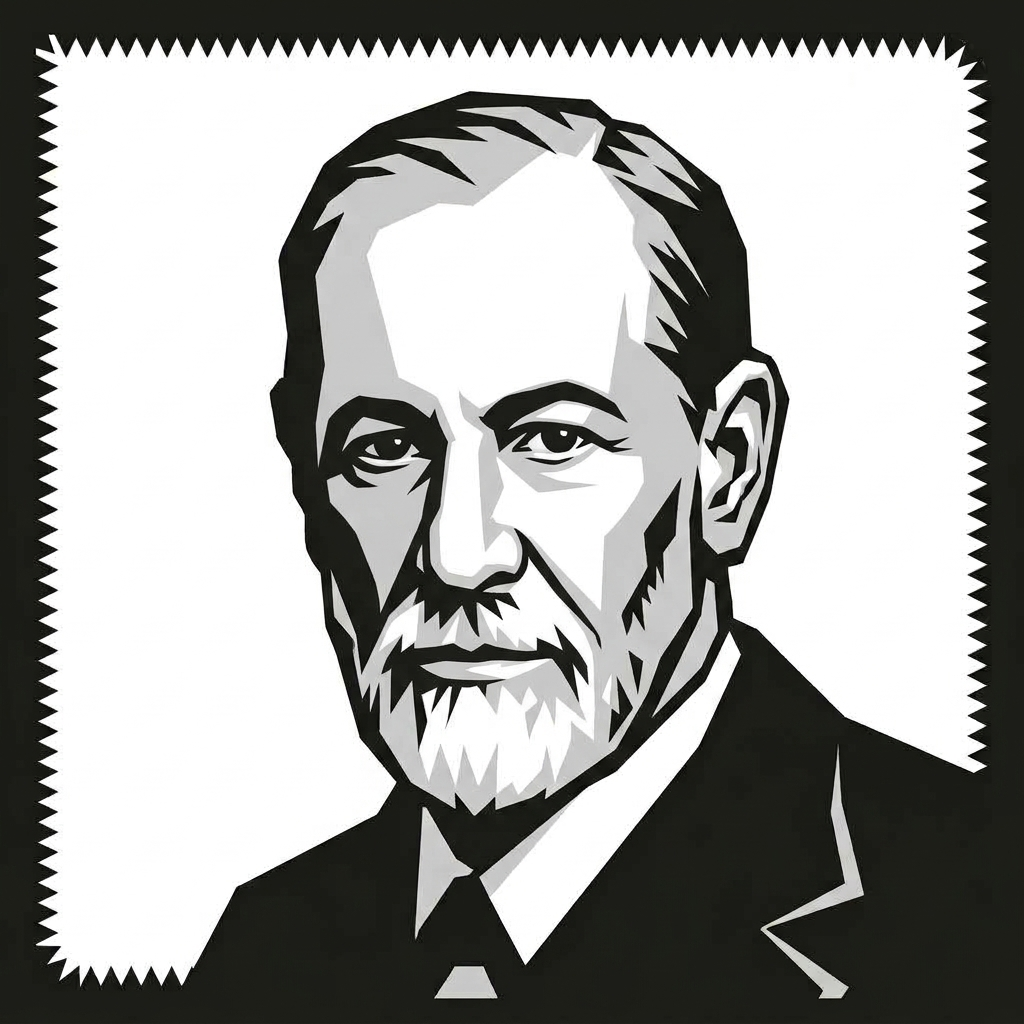
\includegraphics[width=2.1cm]{Freud.png}} 
\end{tabularx}
\end{tcolorbox}

\newpage % ================= SEITE 2: METHODE & ARBEITSAUFTRÄGE =================

\noindent {\Large \textbf{\color{primaryBlue}Arbeitsaufträge \& Methode}}
\vspace{0.25cm}

% === METHODENKASTEN: PLACEMAT-STRUKTURLEGETECHNIK ===
\begin{tcolorbox}[
    enhanced, colback=lightBlue, colframe=primaryBlue, boxrule=0.8pt, arc=1mm,
    title=\textbf{Methode: Placemat-Strukturlegetechnik},
    fonttitle=\small\bfseries\color{white},
    boxed title style={colback=primaryBlue, arc=0mm, boxrule=0pt},
    attach boxed title to top left={yshift=-2mm, xshift=2mm},
    boxsep=5pt, bottom=5pt, top=7pt
]
\small\sffamily
\textbf{Ziel:} Zentrale Begriffe eines philosophischen Textes kriterienorientiert isolieren und im Team zu einer sachlogischen Gedankenarchitektur verbinden.\par\smallskip
\begin{enumerate}[leftmargin=0.5cm, itemsep=0.08cm, topsep=0.02cm]
    \item \textbf{Think (Außenfeld):} Lies den Text aufmerksam. Schreibe 6--8 zentrale Schlüsselbegriffe heraus. Markiere:
    \begin{itemize}[leftmargin=0.4cm, itemsep=0.02cm, label=\color{primaryBlue}\textbullet]
        \item[\textbf{!}] = \textit{zentral / tragend für Freuds Argumentation}
        \item[\textbf{?}] = \textit{unklar / erklärungs- oder diskussionsbedürftig}
    \end{itemize}
    \item \textbf{Pair / Group (Mittelfeld):} Dreht das Placemat, stellt eure Begriffe kurz vor und einigt euch gemeinsam auf die \textbf{5 Kernbegriffe}.
    \item \textbf{Strukturlegen:} Legt die 5 Begriffe als Kärtchen in der Mitte aus und ordnet sie sachlogisch (von der biologischen Triebnatur bis zur seelischen Kostenstelle). Verbindet sie mit beschrifteten Pfeilen ($\rightarrow$, $\leftrightarrow$).
\end{enumerate}
\end{tcolorbox}

\vspace{0.15cm}

% === AUFGABE 1: PLACEMAT-STRUKTURLEGETECHNIK ===
\begin{aufgabe}{\iconEA \, \iconGA}
\textbf{Erschließt} Freuds Argumentationsgang nach der \textit{Placemat-Strukturlegetechnik}:
\begin{enumerate}[label=\alph*), leftmargin=0.5cm, itemsep=0.08cm]
    \item \textbf{Think (Einzelarbeit):} Notiert eure Schlüsselbegriffe mit Kennzeichnung (\textbf{!} bzw. \textbf{?}) in eurem persönlichen Außenfeld auf dem Placemat.
    \item \textbf{Group (Gruppe):} Gleicht die Begriffe im Team ab, einigt euch auf die \textbf{5 tragenden Fachbegriffe} und bringt sie im Mittelfeld des Placemats in eine logische Rangordnung:
\end{enumerate}
\end{aufgabe}

% === SCHEMA: DIE 5 LOGISCHEN STATIONEN ===
\begin{tcolorbox}[
    enhanced, colback=white, colframe=primaryBlue, boxrule=0.7pt, arc=1mm,
    title=\textbf{Gedankenarchitektur: Die 5 Stationen des Kulturkonflikts (Synthese für das Mittelfeld)},
    fonttitle=\footnotesize\bfseries\color{white},
    boxed title style={colback=primaryBlue, arc=0mm, boxrule=0pt},
    attach boxed title to top left={yshift=-2mm, xshift=2mm},
    boxsep=3pt, bottom=4pt, top=6pt
]
\footnotesize\sffamily
\renewcommand{\arraystretch}{1.3}
\begin{tabularx}{\textwidth}{|l|X|}
\hline
\textbf{\color{primaryBlue}1. Biologische Natur:} & \textit{Ausgangszustand des Menschen (Triebbegabung, Verhältnis zum Nächsten)} \vspace{0.15cm} \\
\hline
\textbf{\color{primaryBlue}2. Bedrohte Kultur:} & \textit{Konsequenz für das Zusammenleben (Warum Gesellschaft zerbrechlich ist)} \vspace{0.15cm} \\
\hline
\textbf{\color{primaryBlue}3. Kulturelle Zähmung:} & \textit{Forderung \& Barrieren der Zivilisation (Reaktionsbildung, Liebesgebot)} \vspace{0.15cm} \\
\hline
\textbf{\color{primaryBlue}4. Psychischer Wandel:} & \textit{Der innere Wendepunkt (Wohin weicht die Aggression aus? Instanz)} \vspace{0.15cm} \\
\hline
\textbf{\color{primaryBlue}5. Seelische Kostenstelle:} & \textit{Der psychische Preis der Ordnung (Dauerspannung, Gewissen, Unbehagen)} \vspace{0.15cm} \\
\hline
\end{tabularx}
\end{tcolorbox}

\vspace{0.2cm}

% === AUFGABE 2: SYNTHESE & TRANSFER ===
\begin{aufgabe}{\iconPA}
\textbf{Synthetisiert} Freuds Kulturkritik im Hinblick auf unsere Leitfrage zur \textit{Golden Record}:
\begin{enumerate}[label=\alph*), leftmargin=0.5cm, itemsep=0.08cm]
    \item \textbf{Détournement (Subversive Verfremdung):} Öffnet das Sport-Foto der Schulkinder (NASA-Katalog Nr. 56) auf eurem Tablet. Zeichnet mit dem Stift ein, was Freud \textit{hinter} dieser friedlichen Wettkampfordnung diagnostiziert (z.\,B. Es-Impulse, Ketten des Über-Ichs, nach innen gewendete Aggression).
    \item \textbf{Reihen-Synthese:} Positioniert Freud in eurem digitalen \textit{Advanced Organizer} als Gegenpol zu Arnold Gehlen und formuliert \textbf{genau einen} prägnanten Satz, welcher den seelischen Preis für die institutionelle Entlastung benennt.
\end{enumerate}
\end{aufgabe}

\vspace{\fill}

% === DIDAKTISCHE RESERVE ===
\noindent
\footnotesize \runningMan \, \textbf{\color{primaryBlue}Schnelldenker – Didaktische Reserve (Leistungsdruck \& Meme-Transfer):} \\
\textbf{Beurteilt} kritisch: Lässt sich Freuds Modell des Über-Ichs auf das moderne Phänomen des schlechten Gewissens beim Nichtstun („Hustle Culture“, „5 AM Routine“) übertragen? \textbf{Wer ist hier Richter und wer Angeklagter?}

\end{document}
